\documentclass[12pt,a4paper]{article}
\usepackage[english]{babel}
\usepackage[margin=2.5cm]{geometry} %Global margins :)
\usepackage{graphicx}
\usepackage{nicefrac}
\usepackage[modulo]{lineno}
\usepackage{float}
\usepackage{amsmath}
\usepackage{amssymb}
\usepackage{hyperref}
\usepackage{cleveref}
\usepackage{multirow}
\usepackage{units}
\usepackage[section]{placeins}  %prevent floats from being moved over section headings
\usepackage{amsbsy}  % enable bold greek letters in math mode
\usepackage{booktabs}
\usepackage{authblk}   % manage author/affiliations

\bibliographystyle{plain}

% \textheight 24.0cm
% \topmargin -1cm
% \addtolength{\oddsidemargin}{-.5in}
% \addtolength{\evensidemargin}{-.5in}
% \addtolength{\textwidth}{1in}
%  \parskip 7.2pt

\newcommand{\eV}{\, \mathrm{eV}}

\usepackage{color}
\usepackage[]{hyperref}
\hypersetup{
    pdftitle={SD1500 Efficiency},
    pdfauthor={Brichetto Orquera},  
    bookmarksnumbered=true,     
    bookmarksopen=true,         
    bookmarksopenlevel=2,       
%    colorlinks=true,            
    pdfstartview=Fit,           
    pdfpagemode=UseOutlines,    
    pdfpagelayout=TwoPageRight
}

\usepackage{fancyhdr} %Header with the nice line in the top

\pagestyle{fancy}
\fancyhead[R]{GAP Note XX-YY}
% \fancyhead[L]{P. Gabriel Brichetto O.}
% \fancyfoot[C]{\leftmark}
% \fancyfoot[R]{\thepage}

\renewcommand{\headrulewidth}{1pt}


%%%%%%%%%%%%%%%%%%%%%%%%%%%%%%%%%%%%% Body %%%%%%%%%%%%%%%%%%%%%%%%%%%%%%%%%%%%%


\begin{document}

%TODO Include GAP number before submitting

\title{\textbf{Measurement of the SD1500 efficiency with the SD750}}



\author{Gabriel Brichetto Orquera}
\author{Diego Ravignani}
\affil{\scriptsize ITeDA (CNEA, CONICET, UNSAM), Buenos Aires, Argentina}

\date{\vspace{-2 cm}} %removes the date :)

\maketitle

\vspace{2 pt}
\begin{abstract}
The SD spectrum is reported from an energy at which the trigger efficiency is greater than $97\%$.
We propose a fully experimental method to determine the efficiency of the SD1500 as a function of the energy and the zenith angle using the events detected simultaneously with the SD750. The full efficiency energy threshold we found is $2.5\times10^{18}\eV$, in accordance with the current value used bt the collaboration. We also found that this threshold improves to $10^{18}\eV$ with the ToTd and MoPS triggers and by selecting events with zenith angle below $45^{\circ}$.
\end{abstract}

%%%%%%%%%%%%%%%%%%%%%%%%%%%%%% Introduction %%%%%%%%%%%%%%%%%%%%%%%%%%%%%%%%%%%%

\section{Introduction}

The Surface Detector of the Pierre Auger Observatory consists of three nested triangular arrays of Water Cherenkov Detectors (WCD). The first array to be deployed was the SD1500 which consists in 1600 stations. Later, stations were added among the SD1500 stations to form the SD750 near the Cohihueco site (\cref{fig:SD}). Finally, in 2019 a third array was completed by adding stations with a separation of 433 metres to form the SD433 array of 19 stations to reach lower energies. 

\begin{figure}[]
    \begin{center}
        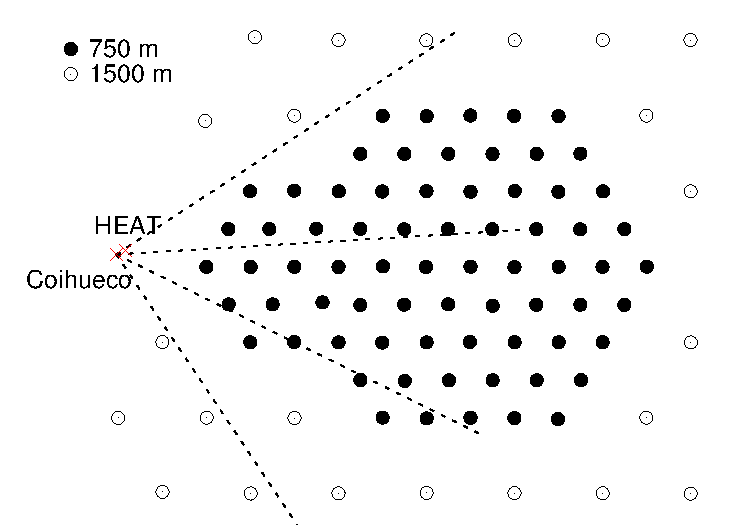
\includegraphics[width=0.5\textwidth]{plots/SD.pdf}  
        \caption{Schematic view of the SD1500 and the SD750 nested within.
        \label{fig:SD}}
        \vspace{-0.5cm}
    \end{center}
\end{figure} 

To measure the spectrum accurately, Auger requires the detector to be fully efficient: the acceptance of the detector must be independent of the mass and energy of the primary cosmic ray. The full efficiency threshold used for practical purposes is $97\%$.
Currently this threshold is measured using the FD by estimating the fraction of hybrid events that also satisfy the SD1500 trigger conditions \cite{Trigger}\cite{VerticalSpectrum}.

Since the SD750 is nested within the SD1500 and has a lower energy threshold, we propose a completely experimental method to study the efficiency for the SD1500. For this we reconstructed the event set of the SD750 and the SD1500 using the rev 33753 of the $\mathrm{\overline{Off}\underline{line}}$ framework. 

For the cosmic ray spectrum, the SD1500 uses events with zenith angle lower than $60^{\circ}$. As a consequence we also studied the zenith angle dependency of the efficiency.

The spectrum is currently reported using only the ToT and TH2 station level triggers \cite{Trigger}. However, in 2014 the ToTd and MoPS triggers were added \cite{Coleman}. These new triggers are designed to be more sensitive to the electromagnetic component of the showers which is more present in the lower energy events. We measured the improvement in the efficiency and the consequent reduction of the energy threshold with the new triggers.

The idea of this work is to study the SD1500 efficiency using that the SD750 is nested within the SD1500. For WCD arrays it is expected that after a certain energy it will be able to detect the signal of the air shower produced by the primary cosmic ray. After that, the efficiency will start to increase and plateau at $100\%$ (full efficiency). The energy at which this occurs will depend on the distance between the stations, the nearer the stations, the lower the energy where full efficiency is reached. But this is a constant compromise with the exposure of the detectors, since the CR flux decays exponentially. In Auger, currently the full efficiency threshold for the SD1500 is taken at $2.5\times10^{18}\eV$ while for the SD750 is $10^{17}\eV$ \cite{SD750Spectrum}. Since the SD750 is fully efficient at the energy range where the SD1500 starts to detect, the SD750 events can be used as a reference and estimate the efficiency by seeing the subset of events mutually detected. For the SD1500 spectrum currently Auger only uses the reconstruction using the original ToT and TH2 triggers, but with the inclusion of the new more sensitive to the electromagnetic component of the shower triggers, it is expected to be able to have a fully efficient detector at a lower energy. 

%%%%%%%%%%%%%%%%%%%%%%%%%%%%%%% Efficiency %%%%%%%%%%%%%%%%%%%%%%%%%%%%%%%%%%%%%

\section{Measurement of the SD1500 efficiency}
\label{sec:efficiency}

In order to compare the efficiency both reconstructing only with the original triggers and including the new triggers, the time period of the analysis ranges from the inclusion of the new triggers, Jan 1st 2014 up to the AMIGA comm crisis, Aug 31st 2018 \cite{GAPAmigaComms}.

The first step was to measure the dependence of the efficiency with the energy. To avoid mismatch between energy bins in the different arrays which would lead to wrong measurements of the efficiency, a robust estimator of the energy of an event was needed. Figure \ref{fig:energy} shows the energy of the SD1500 events as a function of the SD750 energy and the average of each bin. There is no significant bias in the energy range of interest ($10^{17.5}\eV$ to $10^{20}\eV$). As a consequence, the SD750 energy is used as the energy estimator for both detectors.

% Energy vs Energy plot
\begin{figure}[]
    \begin{center}
        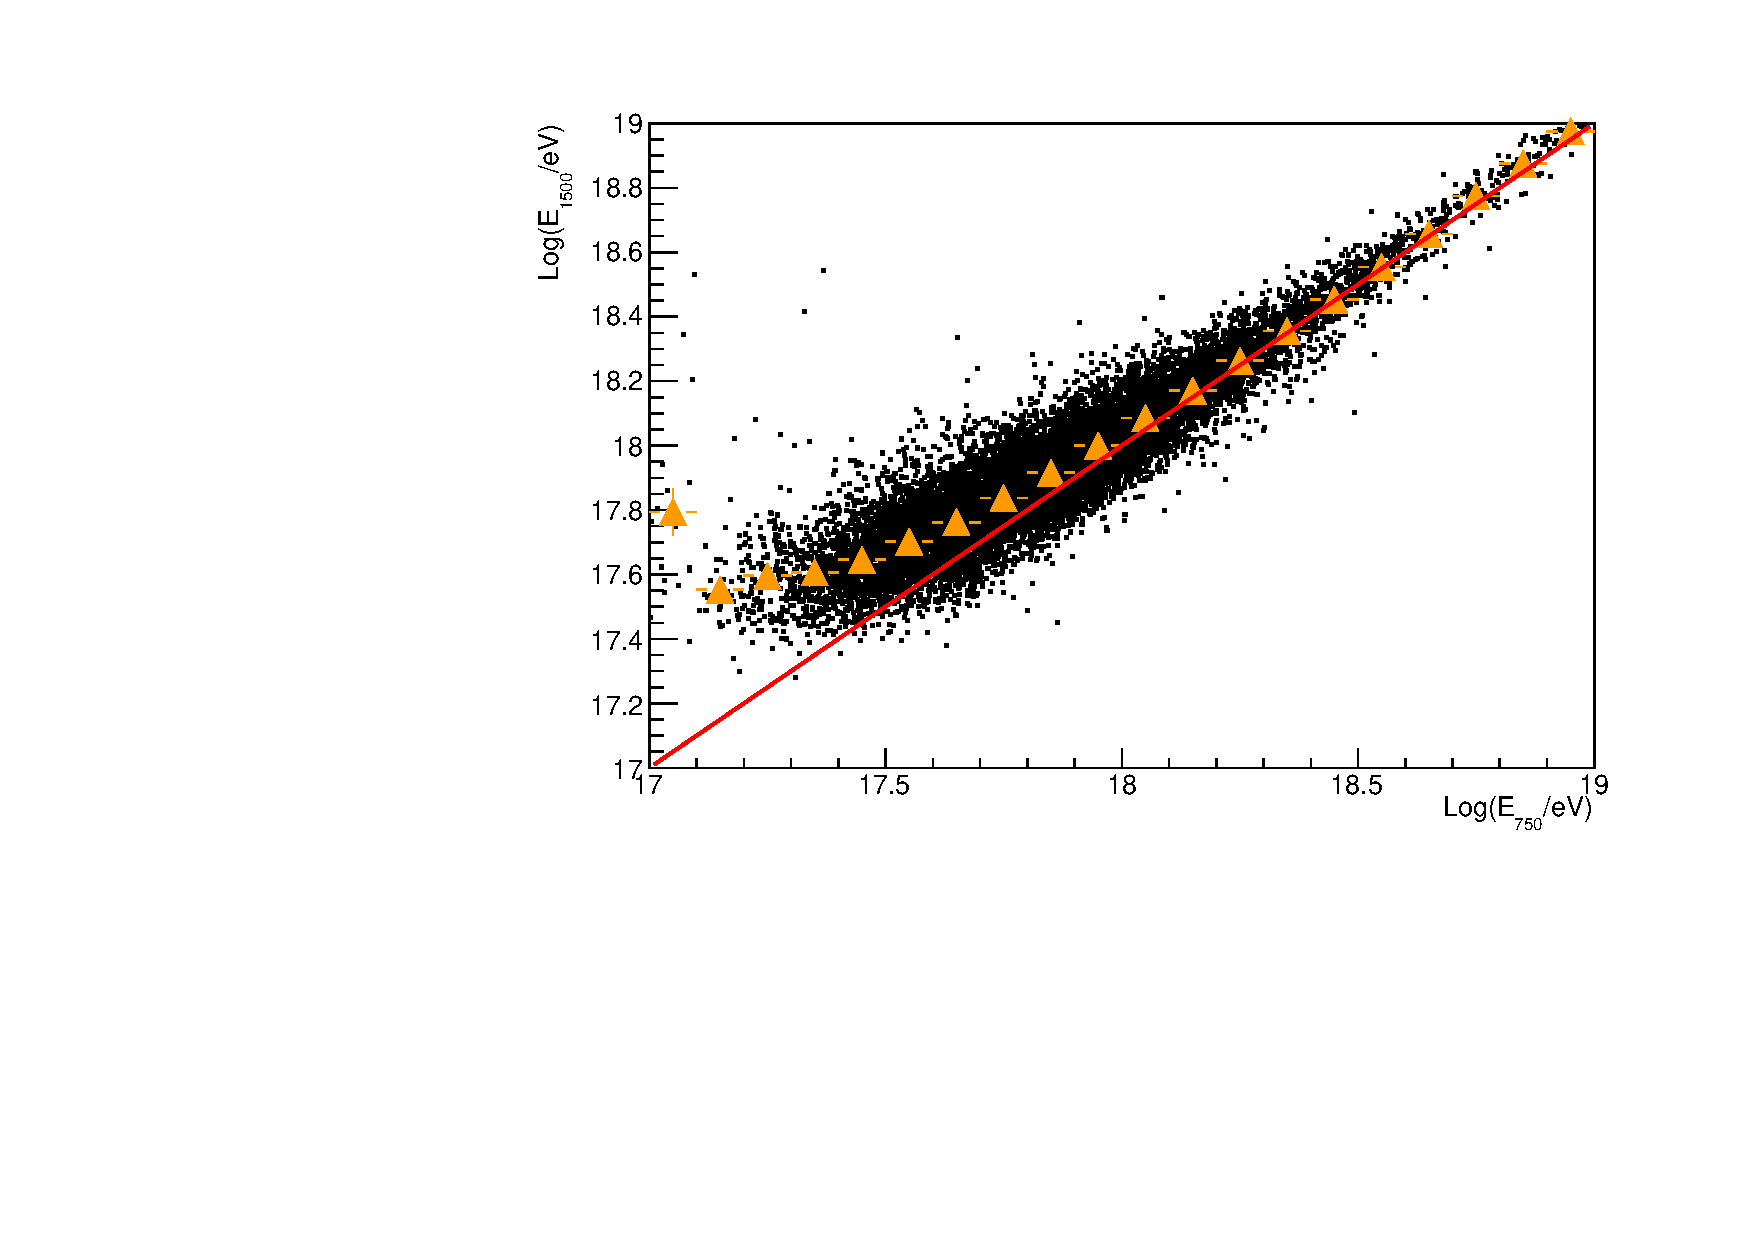
\includegraphics[width=0.6\textwidth]{plots/energy45.pdf}  
        \caption{Energy measured by the SD1500 as a function of the SD750 energy. In red it can be seen the identity function and the bin average.
        \label{fig:energy}}
        \vspace{-0.5cm}
    \end{center}
\end{figure} 

Since the events are independent, the probability of detecting $k$ events with the SD1500 of $n$ SD750 events with success rate $p$ is binomial. In this case, the probability $p$ corresponds to the efficiency of the detector. To estimate the efficiency we used the Maximum Likelihood Estimator (MLE). The likelihood of a binomial distribution is:

\begin{equation}
L(p|n,k)=\binom{N}{k}p^k(1-p)^{n-k}
\label{eqn:Binomial}
\end{equation}

The maximum likelihood estimator $\hat{p}=k/n$ was used as the efficiency estimator, since it is unbiased and with minimum variance. To measure the confidence intervals of the efficiency, the $95\%$ confidence Wilson scored intervals were used, which have a good coverage probability and avoids overshooting when the full efficiency is reached.

First we proceeded with the analysis of the efficiency of the SD1500 including only the original triggers in the whole range of zenith angle. The reconstruction used for vertical events in the SD1500 ranges for $0^{\circ}\leq\theta\leq60^{\circ}$.  Figure \ref{fig:allZenith} shows the efficiency of the SD1500 for zenith angle lower than $60^{\circ}$. 

\begin{figure}[h!]
    \begin{center}
        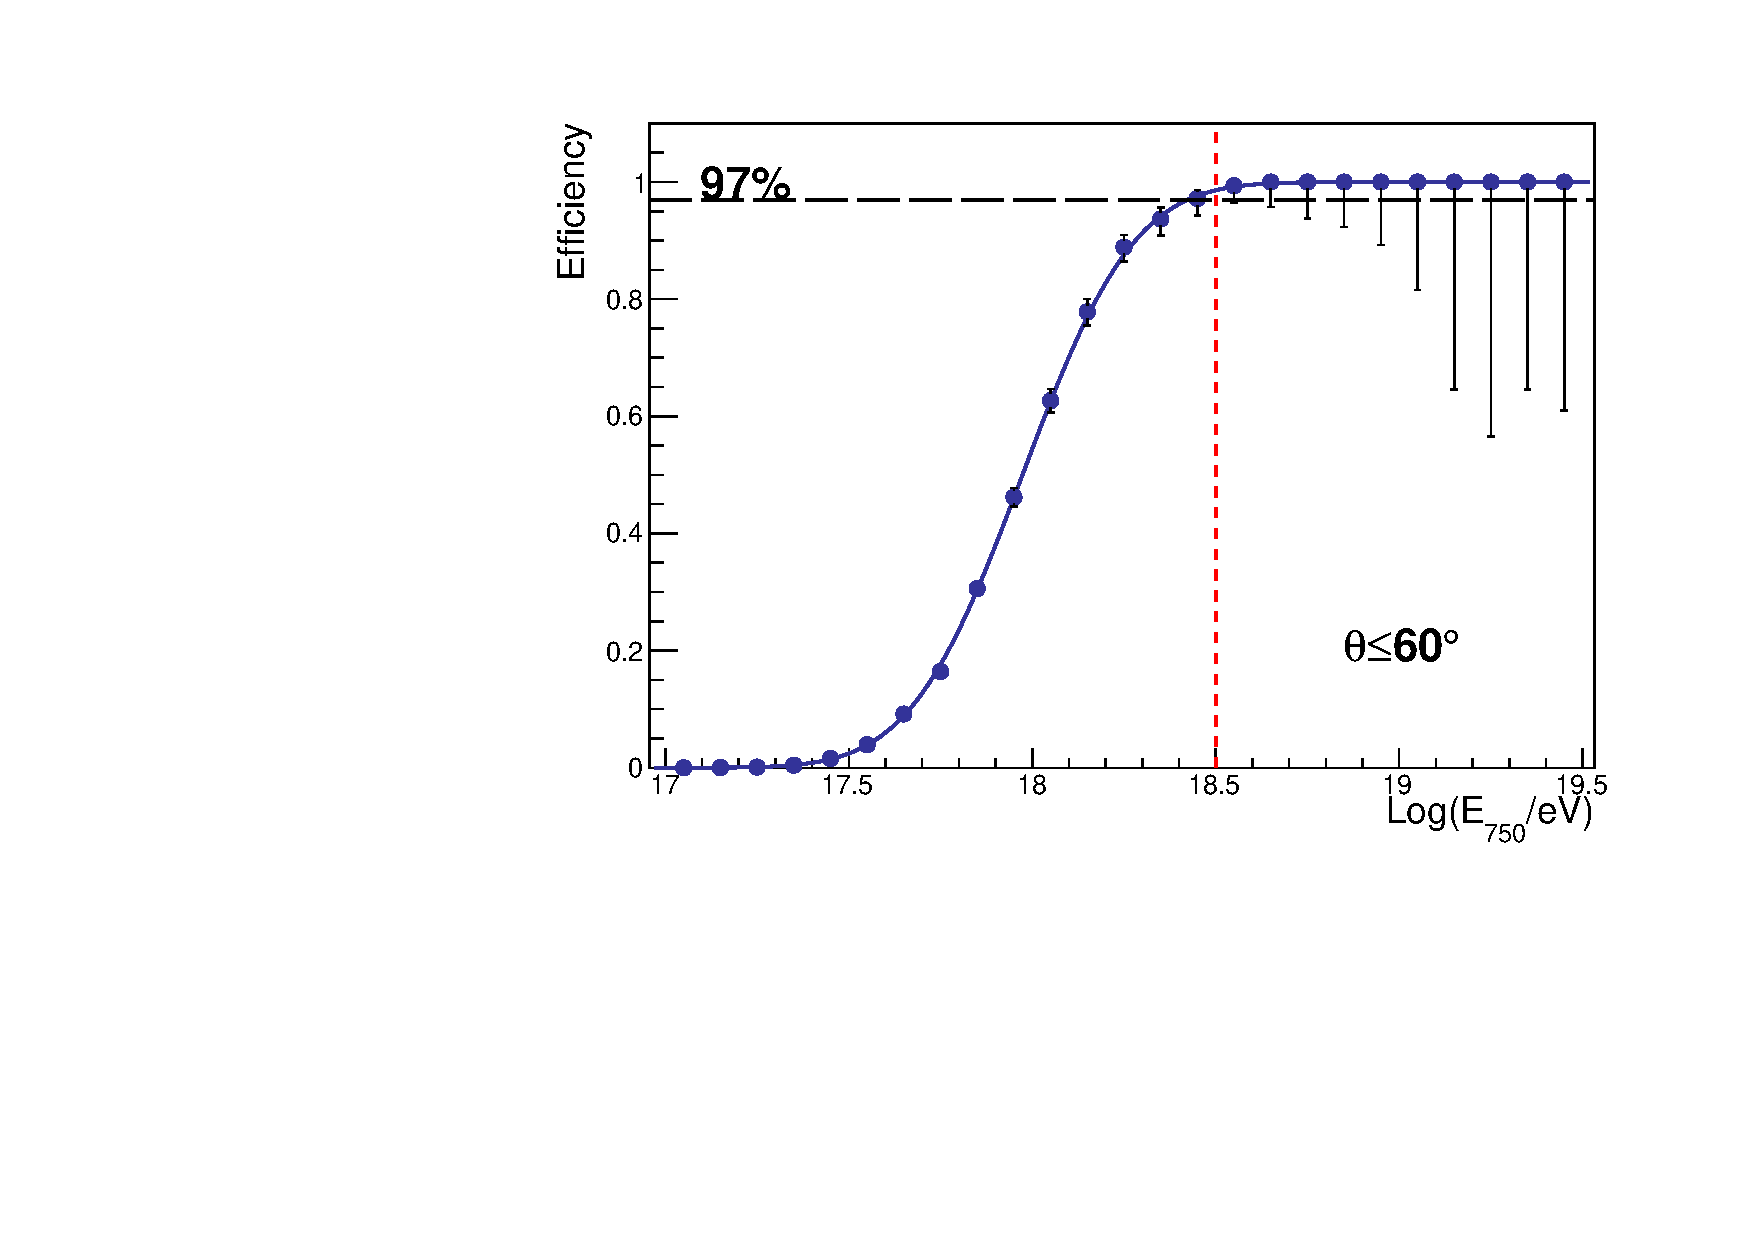
\includegraphics[width=0.6\textwidth]{plots/allZenith.pdf}  
        \caption{SD1500 efficiency measured with the SD750 event set. The error bars show the $95\%$ confidence Wilson score interval. The $97\%$ efficiency threshold is reached at $2.5\times10^{18}\eV$.
        \label{fig:allZenith}}
        \vspace{-0.5 cm}
    \end{center}
\end{figure}

The proposed phenomenological model of the efficiency as a function of the energy is a sigmoid function with two free parameters, $E_0$ and $b$. The election of the error function as the representation of the function is in order to make the results comparable with \cite{VerticalSpectrum}:

\begin{equation}
\varepsilon(E)=\frac{1}{2} + \frac{1}{2}\mathrm{erf}\left(\frac{\log_{10}(E_{750}/\mathrm{eV})-E_{0}}{b}\right)
\label{eqn:Efficiency}
\end{equation}

Using the Minuit routine for a $\chi^2$ method the parameters $E_0=17.97$ and $b=0.393$ were obtained.

For this measurement the threshold $97\%$ efficiency is reached for events with energy higher than $2.5\times10^{18}\eV$ which is in accordance with the current value used by Auger.


%%%%%%%%%%%%%%%%%%%%%%%%%%%%%%Zenith Dependence%%%%%%%%%%%%%%%%%%%%%%%%%%%%%%%%%


\section{Zenith angle dependence of the efficiency}
\label{sec:zenith}

The next step is to analyse the dependency of the efficiency with the zenith angle of the events. We divided the events with zenith angles $\leq60^{\circ}$ in twelve zenith bins equispaced in $\sin^2(\theta)$ in order to have approximately the same exposure. Based on \cite{VerticalSpectrum} we propose a combined model of the efficiency consisting in a sigmoid function, just like \cref{eqn:Efficiency} but including the dependency on the zenith angle in the parameters $E_0$ and $b$:

\begin{equation}
\varepsilon(E,\theta)=\frac{1}{2} + \frac{1}{2}\mathrm{erf}\left(\frac{\log_{10}(E_{750}/\mathrm{eV})-E_{0}(\theta)}{b(\theta)}\right)
\label{eqn:EffiZenith}
\end{equation}

\begin{figure}[h]
    \begin{center}
        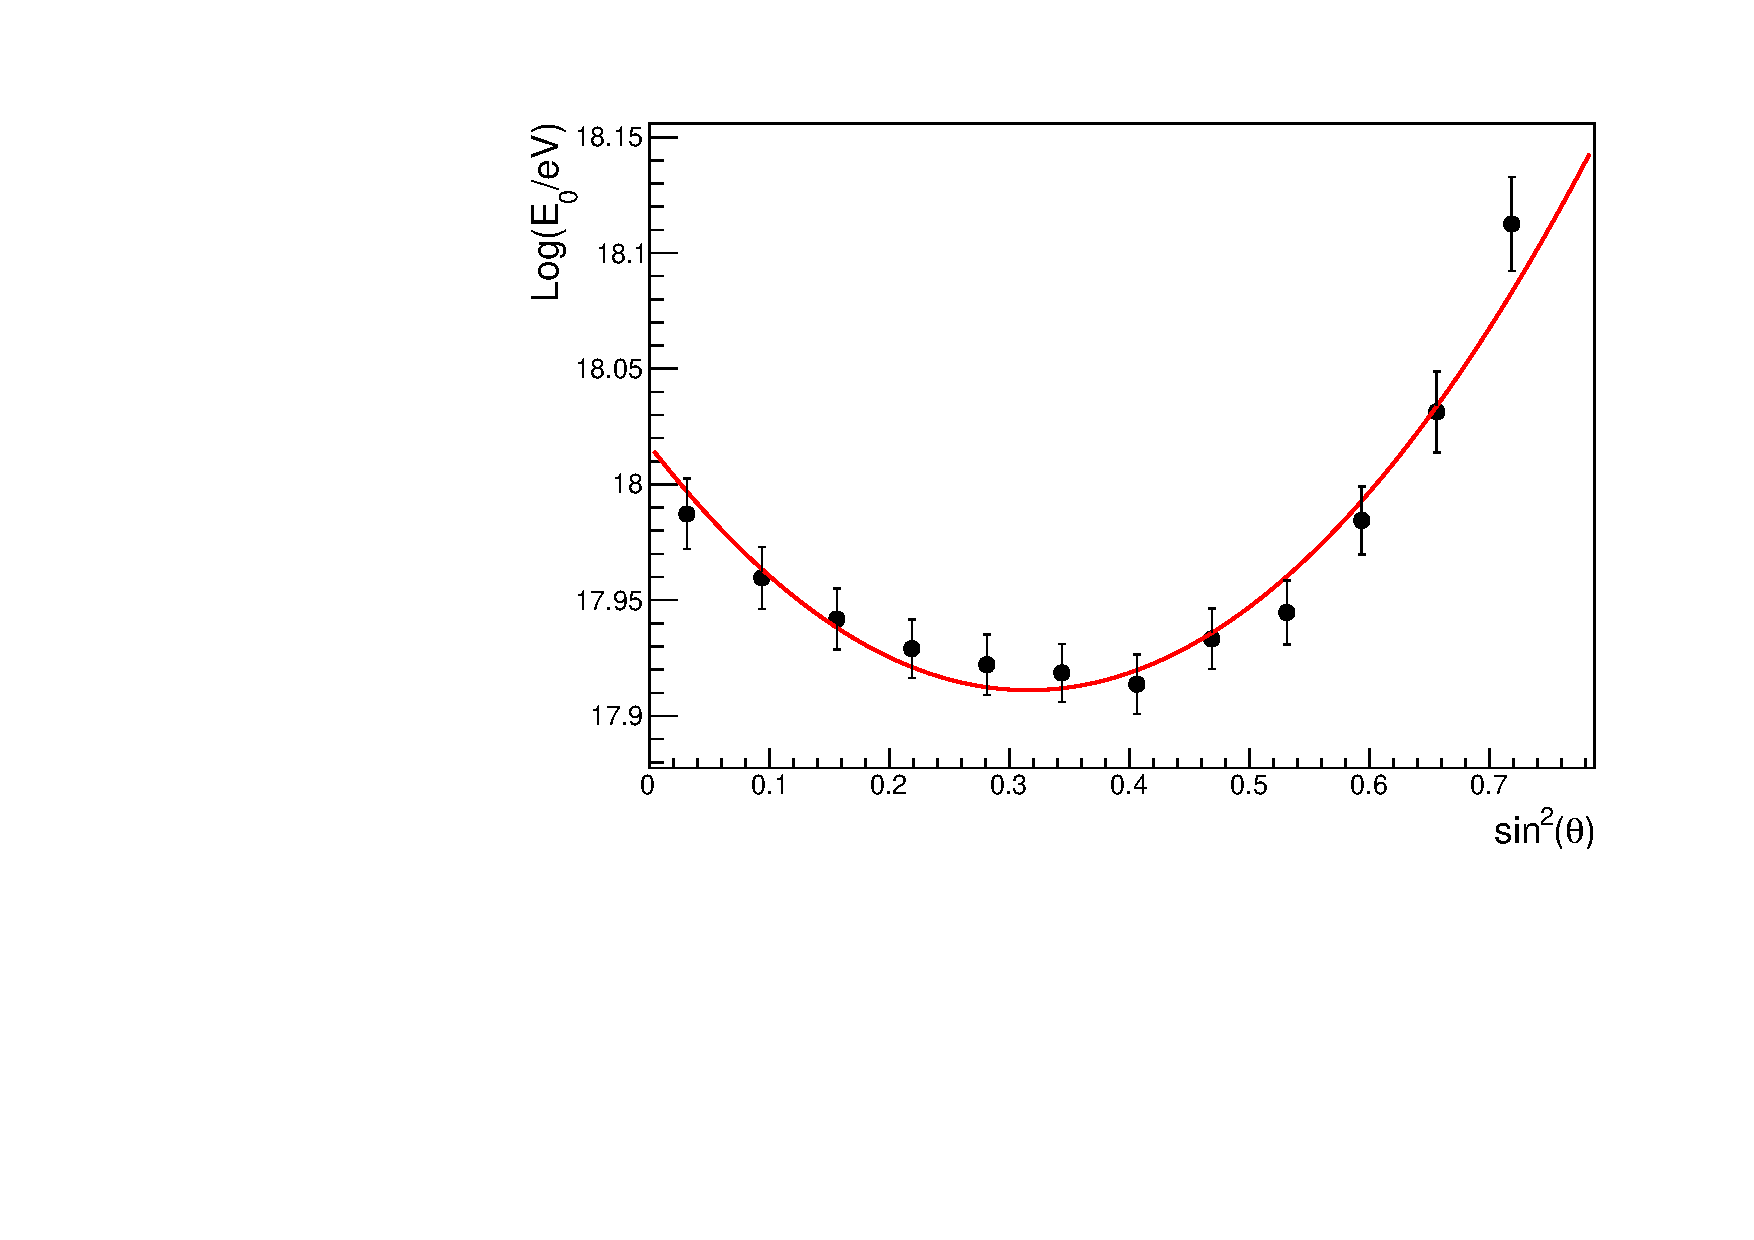
\includegraphics[width=0.49\textwidth]{plots/E0.pdf}
        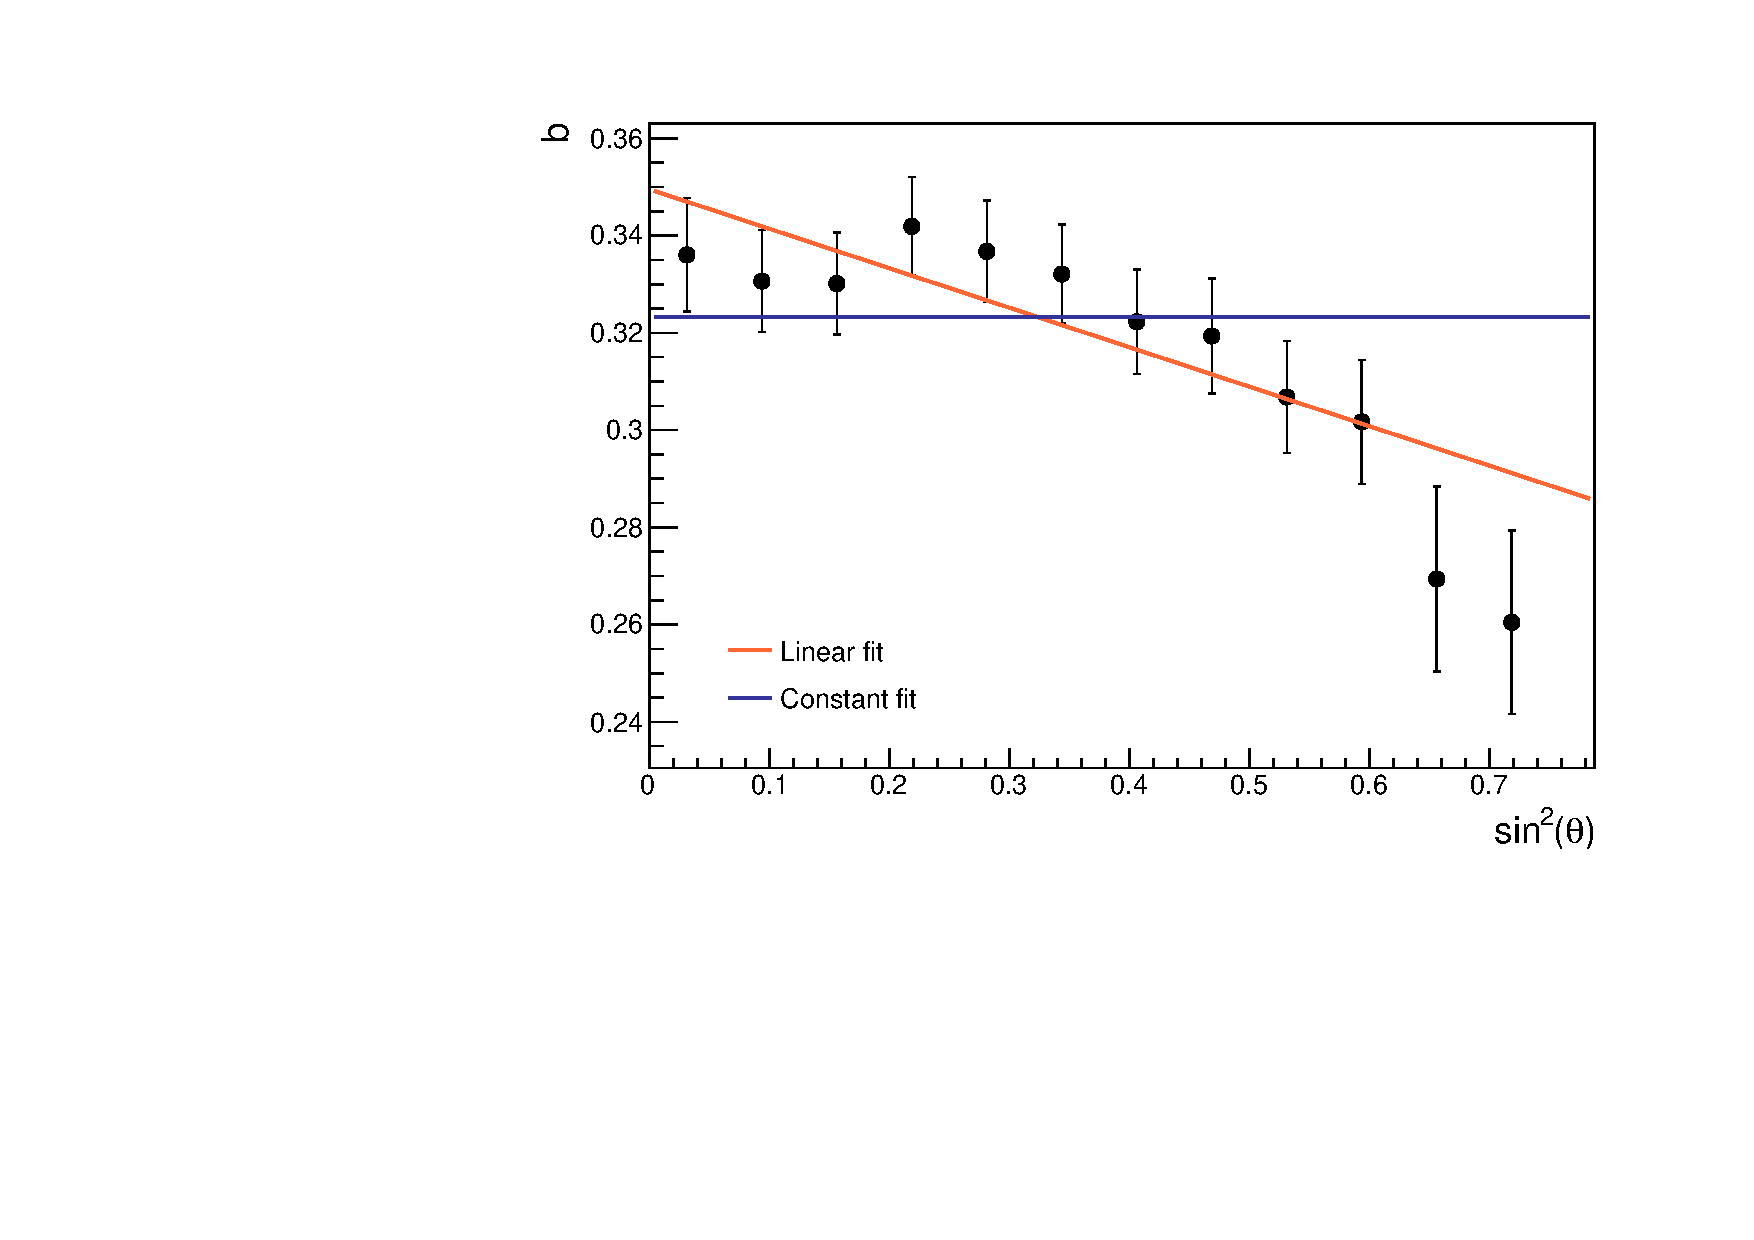
\includegraphics[width=0.49\textwidth]{plots/b.pdf}
        \caption{Parameter dependency with $\sin^2(\theta)$ for the preliminary fit. $E_0$ shows a quadratic dependence and $b$ is modelled by a constant function and a linear function.
        \label{fig:parameters}}
        \vspace{-0.5cm}
    \end{center}
\end{figure} 

In order to see the functional form of $E_0(\theta)$ and $b(\theta)$ we propose a preliminary analysis where the efficiency is measured for each $\sin^2(\theta)$ bin separately. Figure \ref{fig:parameters} shows a quadratic dependency of $E_0$ while for $b$, two models are proposed, one of constant $b$ and other linear in $\sin^2(\theta)$. In consequence two parametrizations of the efficiency as a function of the energy and the zenith angle are proposed: one of 4 parameters with $E_0(\theta)=p_0 + p_1\sin^2(\theta) + p_2\sin^4(\theta)$ and $b=b_0$ and one of 5 parameters with the same $E_0$ but $b=b_0+b_1\sin^2(\theta)$. With the fitted parameters for the single bins as initial values, we made a simultaneous $\chi^2$ fit of the efficiency for the 4 parameter and the 5 parameter models. Results are shown in \cref{tab:parameters}.

\begin{figure}[t]
    \begin{center}
        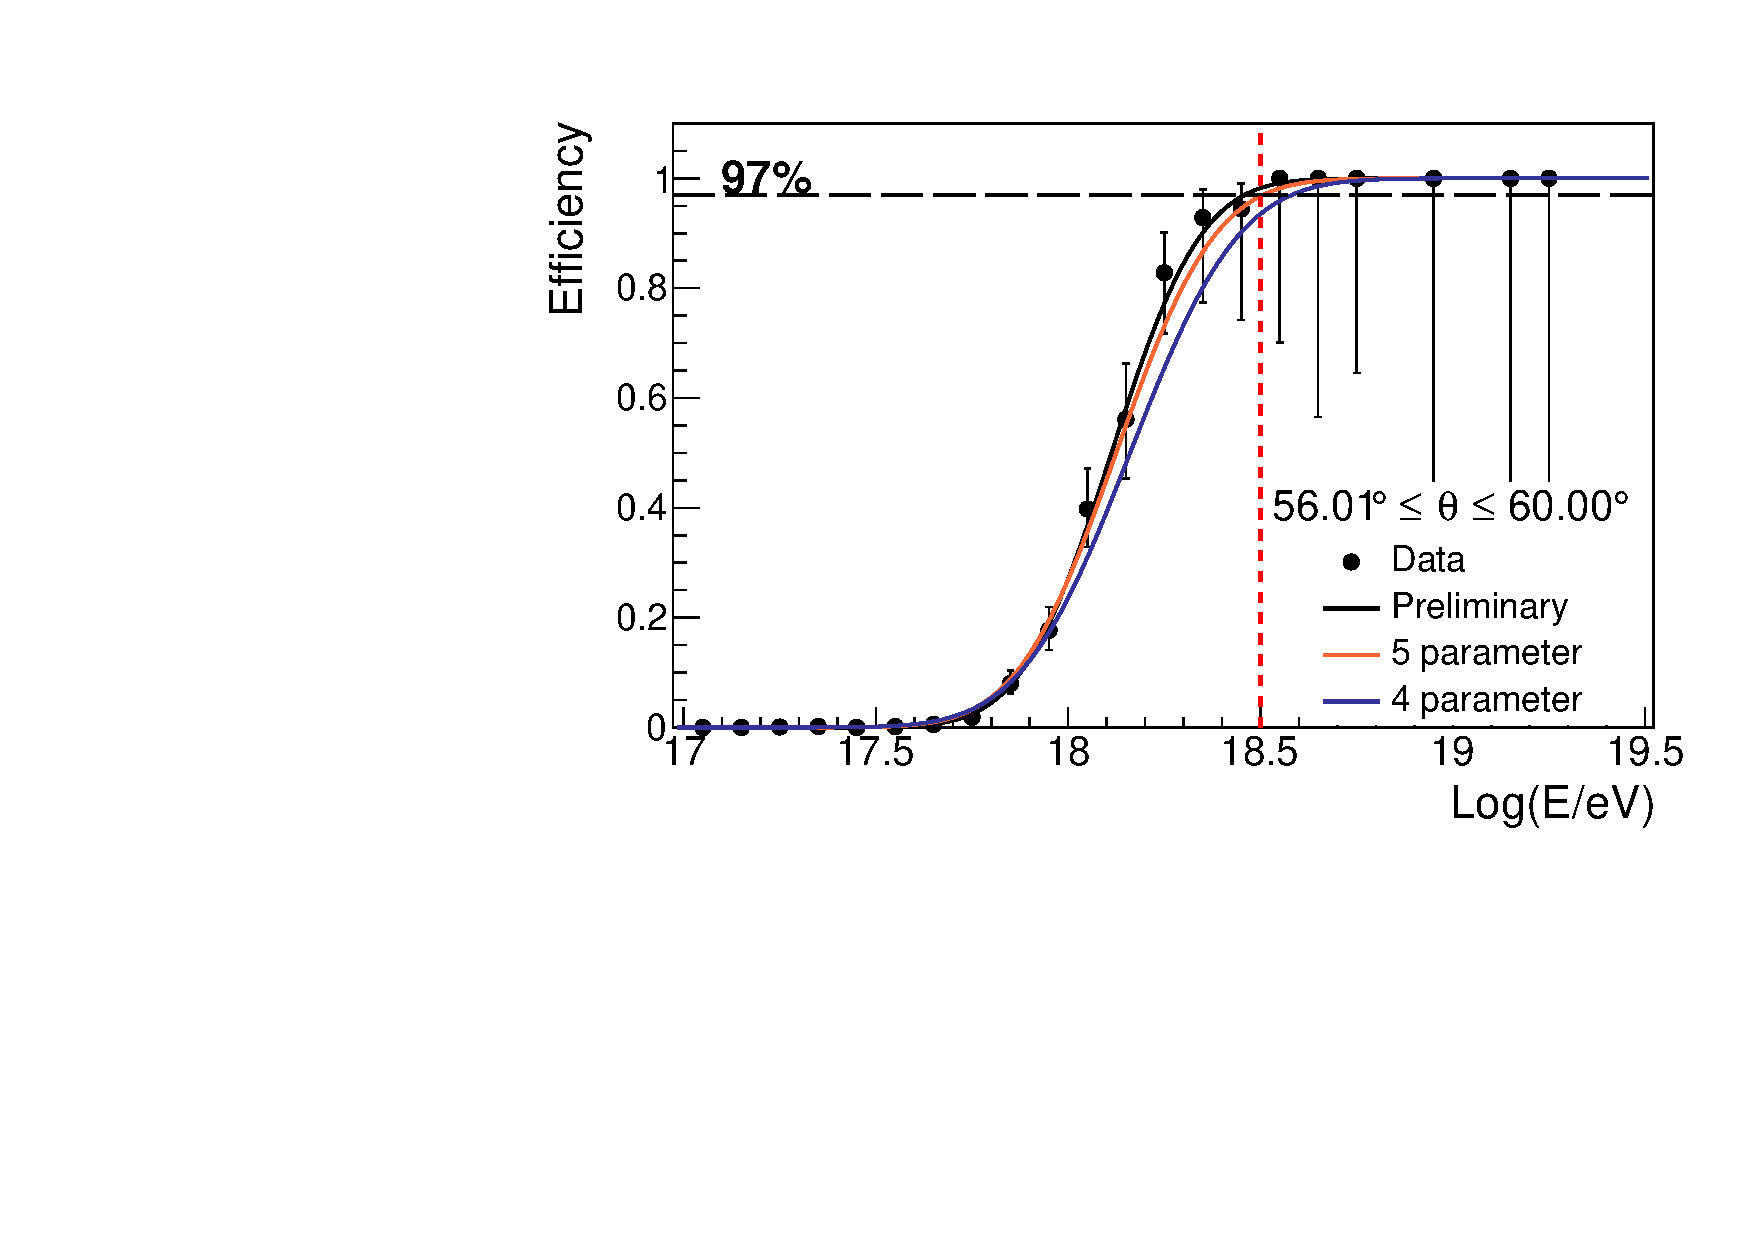
\includegraphics[width=0.6\textwidth]{plots/singleZenithFit.pdf}
        \caption{Efficiency for the $56.0^{\circ}-60.0^{\circ}$ zenith angle bin together with the preliminary fit and the 4 and 5 parameter models.
        \label{fig:zenithSingle}}
        \vspace{-0.5cm}
    \end{center}
\end{figure}

In order to compare the results, the 4 and 5 parameter fits were evaluated in the centre of each zenith angle bin. As an example, \cref{fig:zenithSingle} shows the results for the bin $56.0 \leq \theta \leq 60.0$. For further reference, \cref{fig:zenith} in the appendix shows this data for all the zenith angle bins. For the more vertical bins, both the 4 and 5 parameter fits show accordance with the measured efficiency but for the more inclined events, the 5 parameter description adjust better the data. Seeing \ref{tab:parameters} can give an explanation for this. Both parameters in the 5 parameter and 4 parameter fits are very similar, the extra linear term in $\sin^2(\theta)$ can be seen as a correction that's specially relevant for the more inclined events. In consequence, our proposed model of the efficiency is the 5 parameter one:

\begin{equation}
\varepsilon(E,\theta)=\frac{1}{2}\left(1+\mathrm{erf}\left(\frac{\log_{10}(E/\mathrm{eV})-(p_0+p_1\sin^2(\theta)+p_2\sin^4(\theta))}{b_0+b_1\sin^2(\theta)}\right)\right)
\label{eqn:fitting}
\end{equation}

with $p_0=18.03$ $p_1=-0.91$, $p_2=1.45$, $b_0=0.336$, $b_1=-0.068$. We are working to have a better understanding of the errors associated with this adjustment.


\begin{figure}[H]
    \begin{center}
        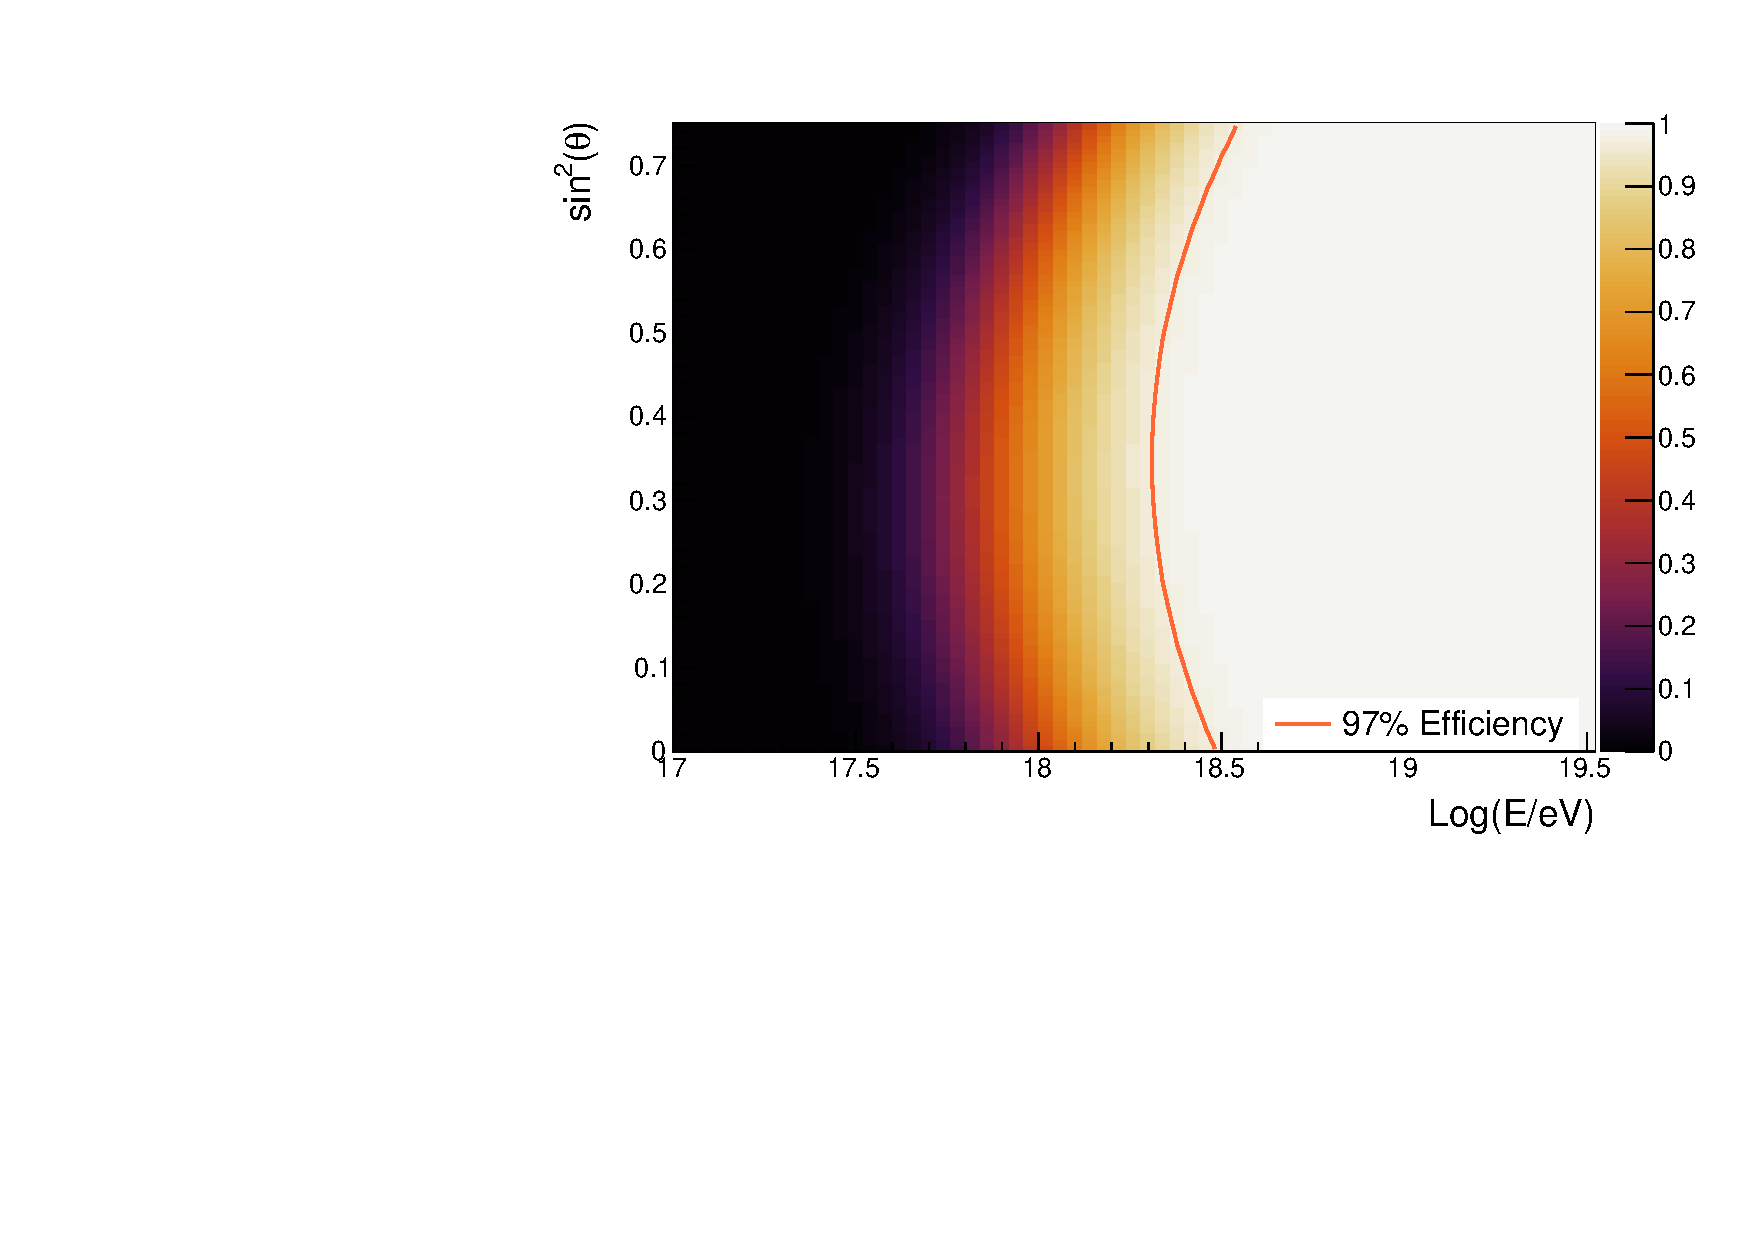
\includegraphics[width=0.6\textwidth]{plots/Surface.pdf}
        \caption{Efficiency as function of the Energy and zenith angle and the $97\%$ surface level.
        \label{fig:surface}}
        \vspace{-0.5cm}
    \end{center}
\end{figure}

Figure \ref{fig:surface} shows the surface plot of the efficiency as a function of the energy and the zenith angle. The efficiency is lower for the vertical events, increasing and reaching a maximum at approximately $30^{\circ}$ and then decreasing for the most inclined events. The $97\%$ efficiency threshold ranges from $10^{18.5}\eV$ improving to almost $10^{18.3}\eV$ at $30^{\circ}$ and then decreases. This behaviour is in accordance to the model proposed in \cite{VerticalSpectrum}.

\begin{table}[H]
\begin{center}
\begin{tabular}{l|ccccc}
        & \textbf{$p_0$} & \textbf{$p_1$} & \textbf{$p_2$} & \textbf{$b_0$} & \textbf{$b_1$} \\ \hline
\textbf{Preliminar}  & $18.01$        & $-0.67$        & $1.1$          & $0.350$        & $-0.08$        \\
\textbf{5 parameter} & $18.03$        & $-0.92$        & $1.45$         & $0.336$        & $-0.07$        \\
\textbf{4 parameter} & $18.01$        & $-0.83$        & $1.44$         & $0.315$        & -             
\end{tabular}
\end{center}
\caption{Parameter results for the preliminary analysis and the 4 and 5 parameter models proposed.}
\label{tab:parameters}
\end{table}


%%%%%%%%%%%%%%%%%%%%%%%%%%%%%%New Triggers%%%%%%%%%%%%%%%%%%%%%%%%%%%%%%%%%%%%%%%%

\section{Inclusion of the ToTd and MoPS triggers}
\label{sec:new}

Since 2013 two new station level triggers were included in the acquisition system for the surface detectors of the Pierre Auger Observatory. However, the SD1500 spectrum currently reconstructs events only using the original ToT and TH2 triggers. These triggers are more sensitive to the electromagnetic component of the shower which is more dominant at lower energies. Since our method is limited only by the full efficiency threshold of the SD750, we propose to use our analysis for the SD1500 dataset reconstructed including these electromagnetic triggers.
In order to do that, the events were reconstructed using the Trunk version 33753 of the Offline framework for the same time period. This reconstruction results in 74853 simultaneous events in both SD arrays, a $500\%$ increase with respect to the reconstruction only with the old triggers.

\begin{figure}[h]
    \begin{center}
        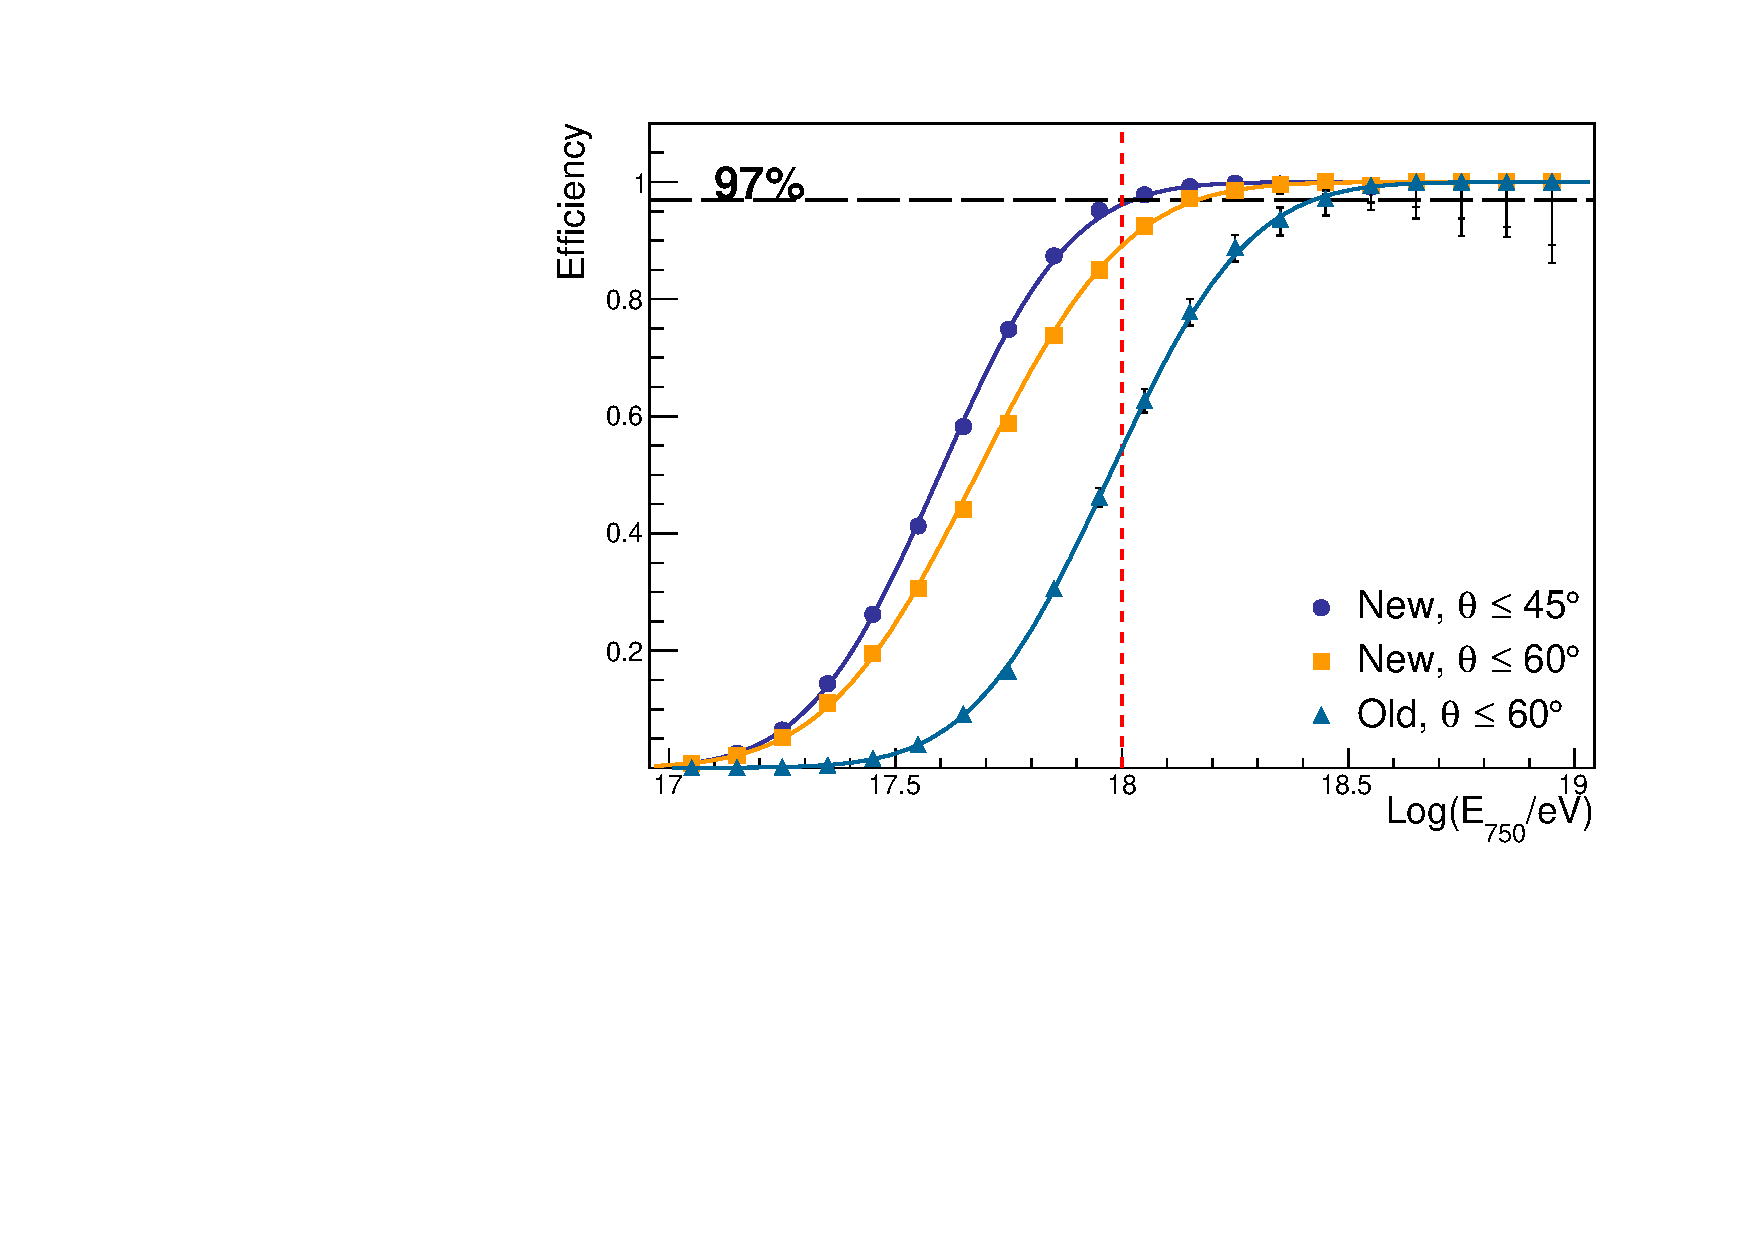
\includegraphics[width=0.7\textwidth]{plots/NewCut.pdf}
        \caption{SD1500 efficiency including the new triggers for $\theta\leq60^\circ$ and $\theta\leq45^\circ$. The $97\%$ efficiency threshold is reached at $10^{18.2}\eV$ and $10^{18}\eV$ respectively.
        \label{fig:NewCut}}
        \vspace{-0.5cm}
    \end{center}
\end{figure}

When including the new triggers in the whole zenith range, from $0^{\circ}$ to $60^{\circ}$ the efficiency increases and the full efficiency starts at $1.25\times10^{18}\eV$, three energy bins lower than using only the original triggers. When the zenith angle dependency is brought into consideration, the efficiency shows a stronger dependency with the inclusion of the new triggers. This is expected, since the electromagnetic component of the shower suffer stronger attenuation because of the further distance travelled in the atmosphere. From this, we propose a modification in the acceptance angle for the events, lowering the maximum zenith angle to $45^{\circ}$. Figure \ref{fig:NewCut} shows the efficiency including the new triggers with and without the new acceptance angle, compared to the reconstruction only including the original triggers. This modification yields to being able to report the spectrum from $10^{18}\eV$, gaining four bins with respect to the current spectrum measurements.

%%%%%%%%%%%%%%%%%%%%%%%%%%%%Spectrum%%%%%%%%%%%%%%%%%%%%%%%%%%%%%%%%%%%%%%%%%


\section{Efficiency correction of the SD1500 Spectrum}
\label{sec:spectrum}

The spectrum measured by Auger with the SD1500 is reported only including events where the acceptance of the detector is independent of the mass and energy of the primary particle. However, having a fully experimental measurement of the energy, we propose to introduce an efficiency correction to the SD1500 spectrum in order to gain data for the lower energies.
Using our reconstructions made for the efficiency analysis, we made the event histogram of the SD1500 for the original triggers and zenith angle below $60^{\circ}$. Also, we made the same histogram for including the new triggers with the new $45^{\circ}$ acceptance angle. To make the histograms comparable, we used as a reference the SD750 event histogram. In first place, the histogram including the new triggers was scaled by 1.5 to have into account the difference of angular exposure with respect to the original triggers histogram. Then, the efficiency correction was introduced by dividing the number of events in each bin by the efficiency measured for that bin. Lastly, all fluxes were scaled to match the flux of the SD750 at $10^{18.4}\eV$, where the detectors are fully efficient to take into account de geometric factors. 

\begin{figure}[h]
    \begin{center}
        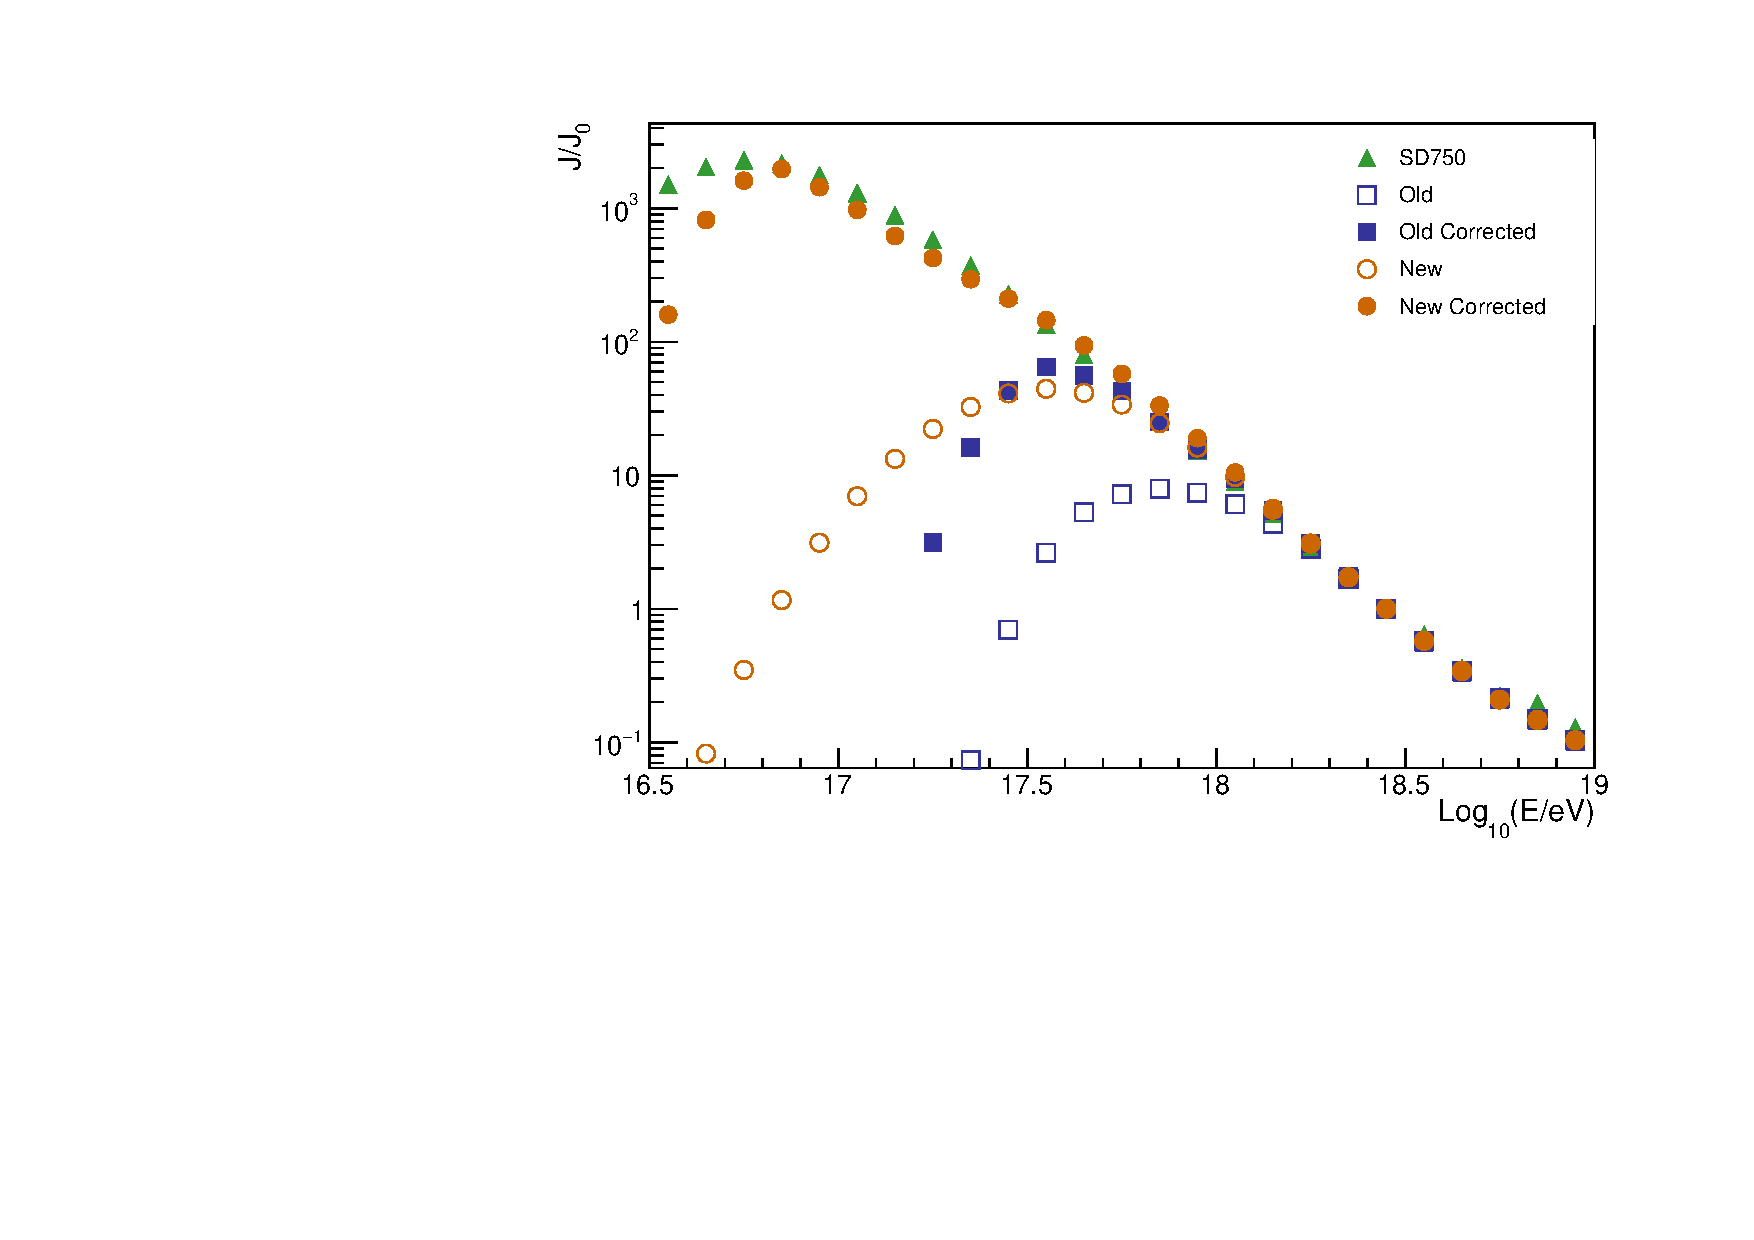
\includegraphics[width=0.7\textwidth]{plots/spectrum.pdf}
        \caption{Raw flux measured by the SD1500 using old and new triggers and it's efficiency correction. The fluxes were normalized to $J_{18.2}=1$.
        \label{fig:flux}}
        \vspace{-0.5 cm}
    \end{center}
\end{figure}

Figure \ref{fig:flux} shows the fluxes both before and after the efficiency correction was introduced. For energies above the full efficiency threshold, the SD1500 fluxes before the correction behave like the SD750. However, for energies below the full efficiency the difference between the measurements quickly increases. With the introduction of the efficiency correction, the SD1500 follows the behaviour of the SD750 for energies lower than full efficiency until the correction factor is too big to have a good estimation of the flux.
For the SD1500 including the new triggers the results are very remarkable, the fluxes being similar for energies as low as $10^17{\eV}$. The relative difference between the flux of the SD1500 and the SD750 is shown in \cref{fig:difference} both before and after the efficiency correction. This preliminary analysis for a possible improvement of the SD1500 spectrum for lower energies shows very promising results. The difference between the fluxes for energies lower than $10^{18}\eV$ increases up to about $100\%$ at $10^{17}\eV$ if it is not corrected. However with the inclusion of the correction the data shows differences of about $25\%$ for this energy range. 

\begin{figure}[H]
    \begin{center}
        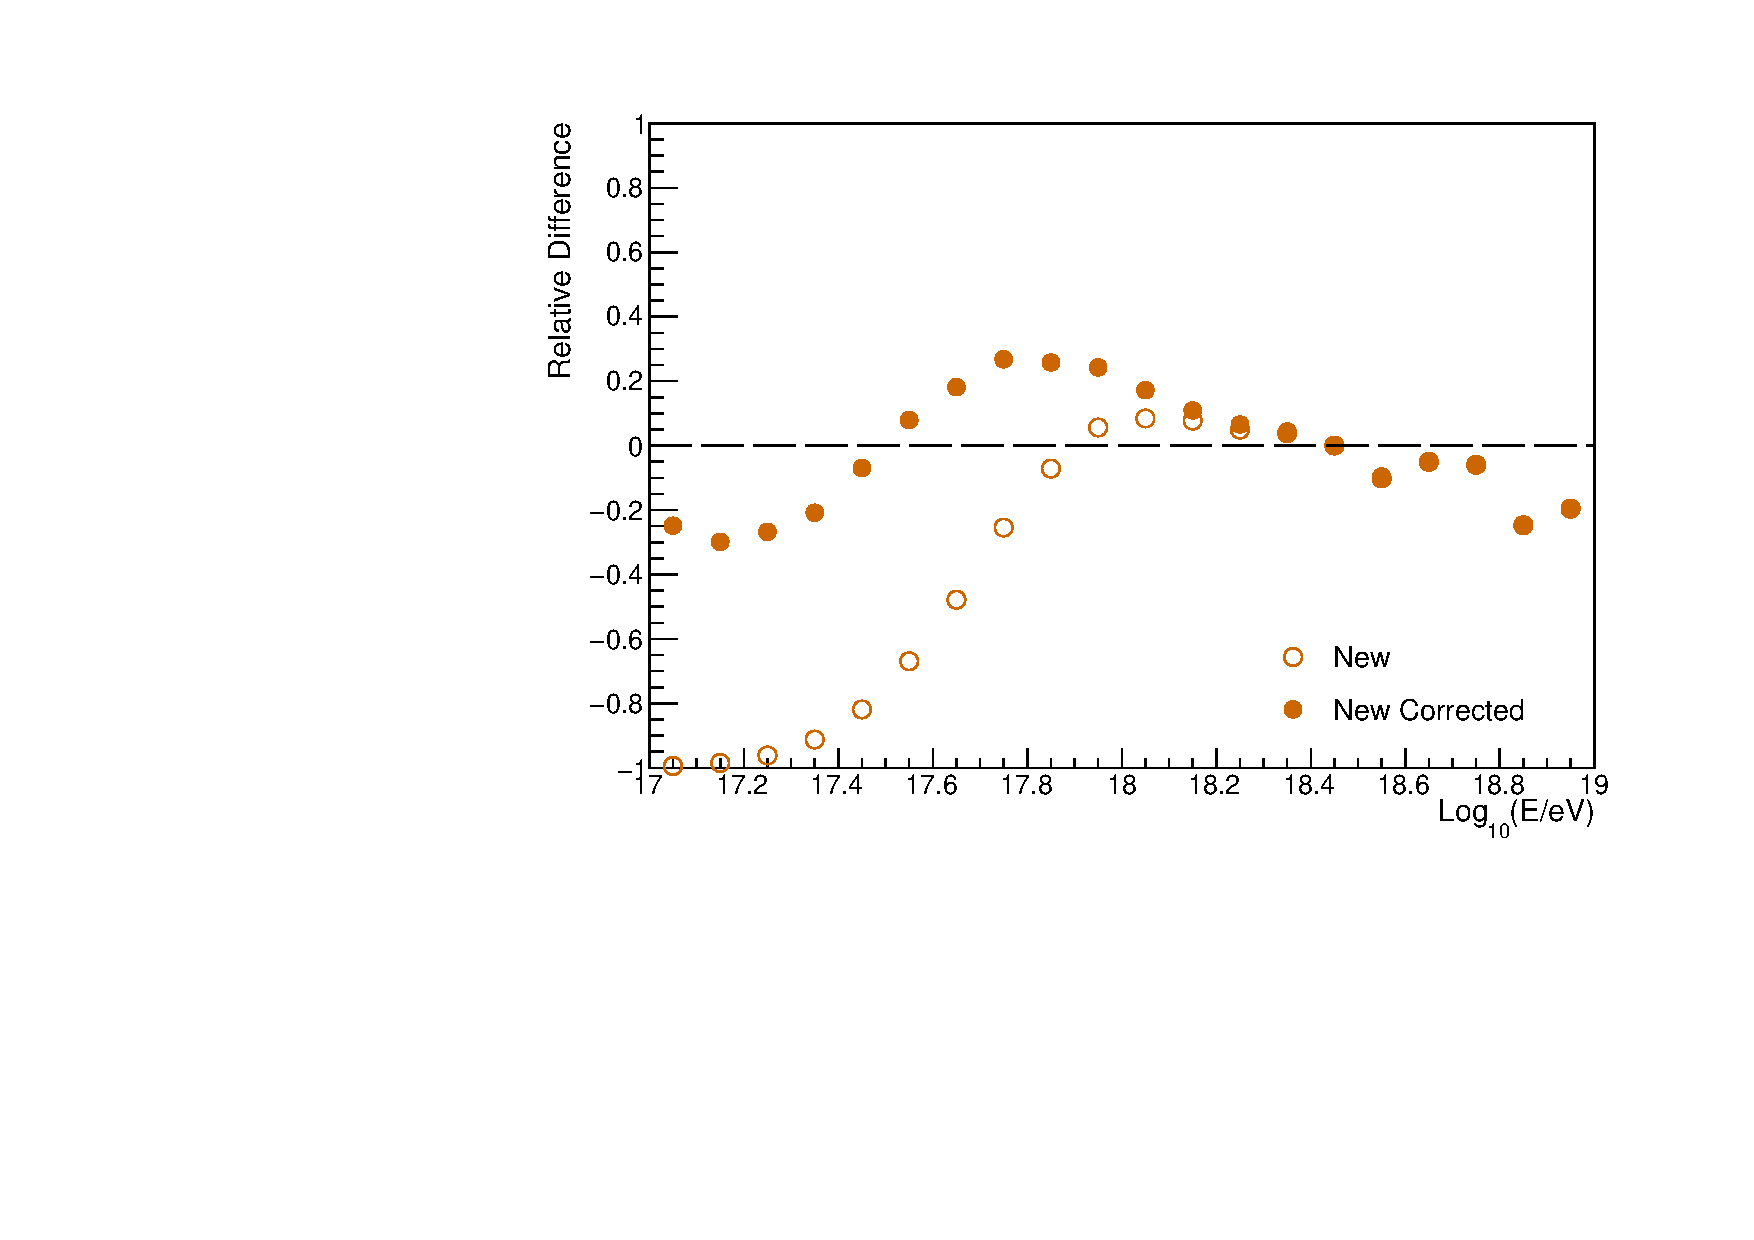
\includegraphics[width=0.7\textwidth]{plots/NewDifference.pdf}
        \caption{Relative difference between SD1500 flux and the SD750 for the old trigger reconstruction and after efficiency correction.
        \label{fig:difference}}
        \vspace{-0.5cm}
    \end{center}
\end{figure} 

\section*{Conclusions}

We provide a fully experimental measurement of the SD1500 efficiency using the SD750 dataset. The efficiency measured shows that the detector acceptance becomes independent of the mass and energy of the primary particle for events with energies higher than $2.51\times10^{18}\eV$ which is in accordance with the current threshold used by Auger. By studying the dependence of the efficiency as a function of the energy and zenith angle we propose a 5 parameter model of the efficiency.
When including the new station level triggers in the reconstruction the efficiency improves and the $97\%$ efficiency threshold is reached for energies above $1.4\times10^{18}\eV$. However, given the stronger dependence of the efficiency on the zenith angle, we propose a new acceptance angle of $45^{\circ}$ which leads to a spectrum starting at $10^{18}\eV$.
Finally we propose the tentative inclusion of an efficiency correction to the SD1500 in order to report the spectrum to even lower energies, having satisfactory results for energies even in the $3.16\times10^{17}\eV$ range.

\pagebreak

\section*{Appendix: Zenith angle dependency of the Efficiency}

\begin{figure}[H]
    \center
    \makebox[\textwidth][c]{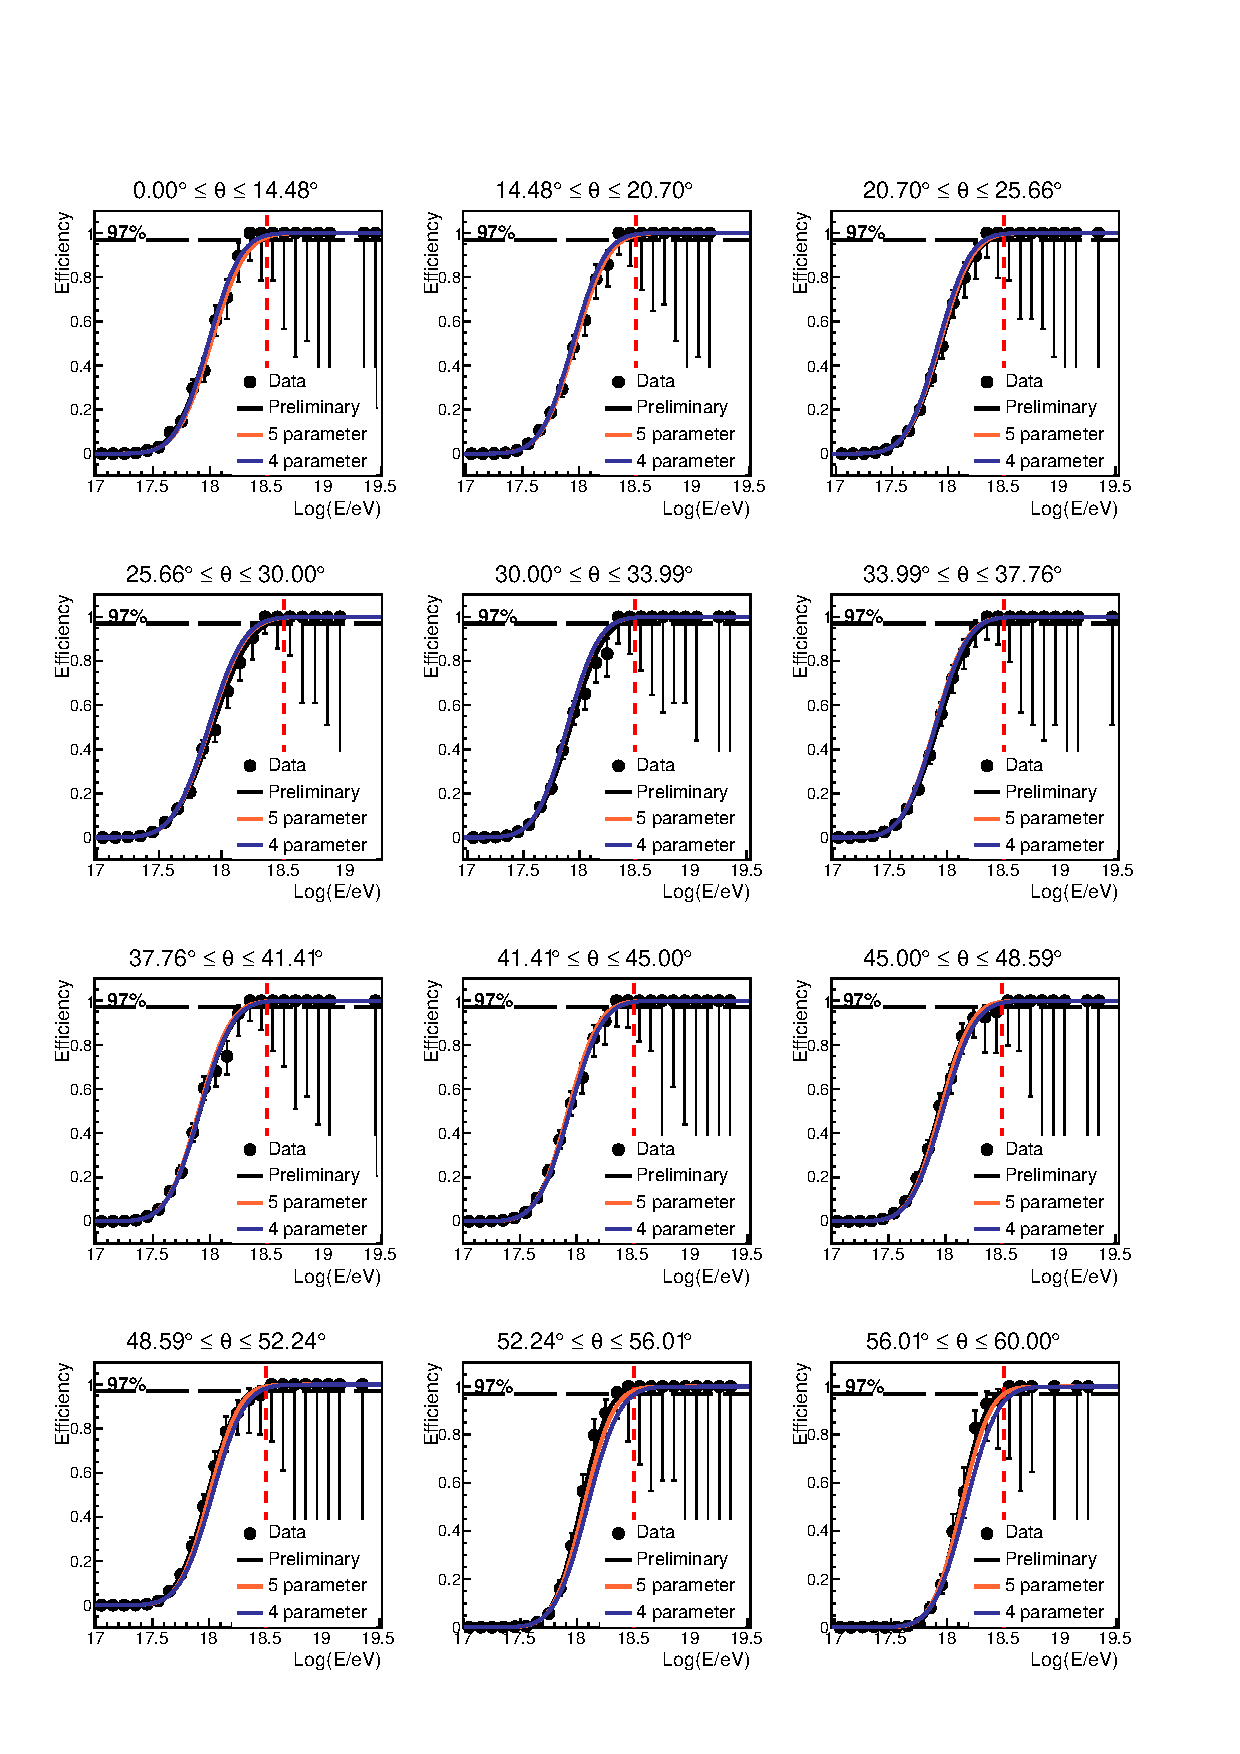
\includegraphics[height=0.9\textheight]{plots/EfficiencyZenith.pdf}}
    \caption{SD1500 efficiency for zenith angle bins and the 4 and 5 parameter fittings proposed together with the preliminary fit.
    \label{fig:zenith}}
\end{figure}

\begin{figure}[p]
    \begin{center}
       \makebox[\textwidth][c]{ 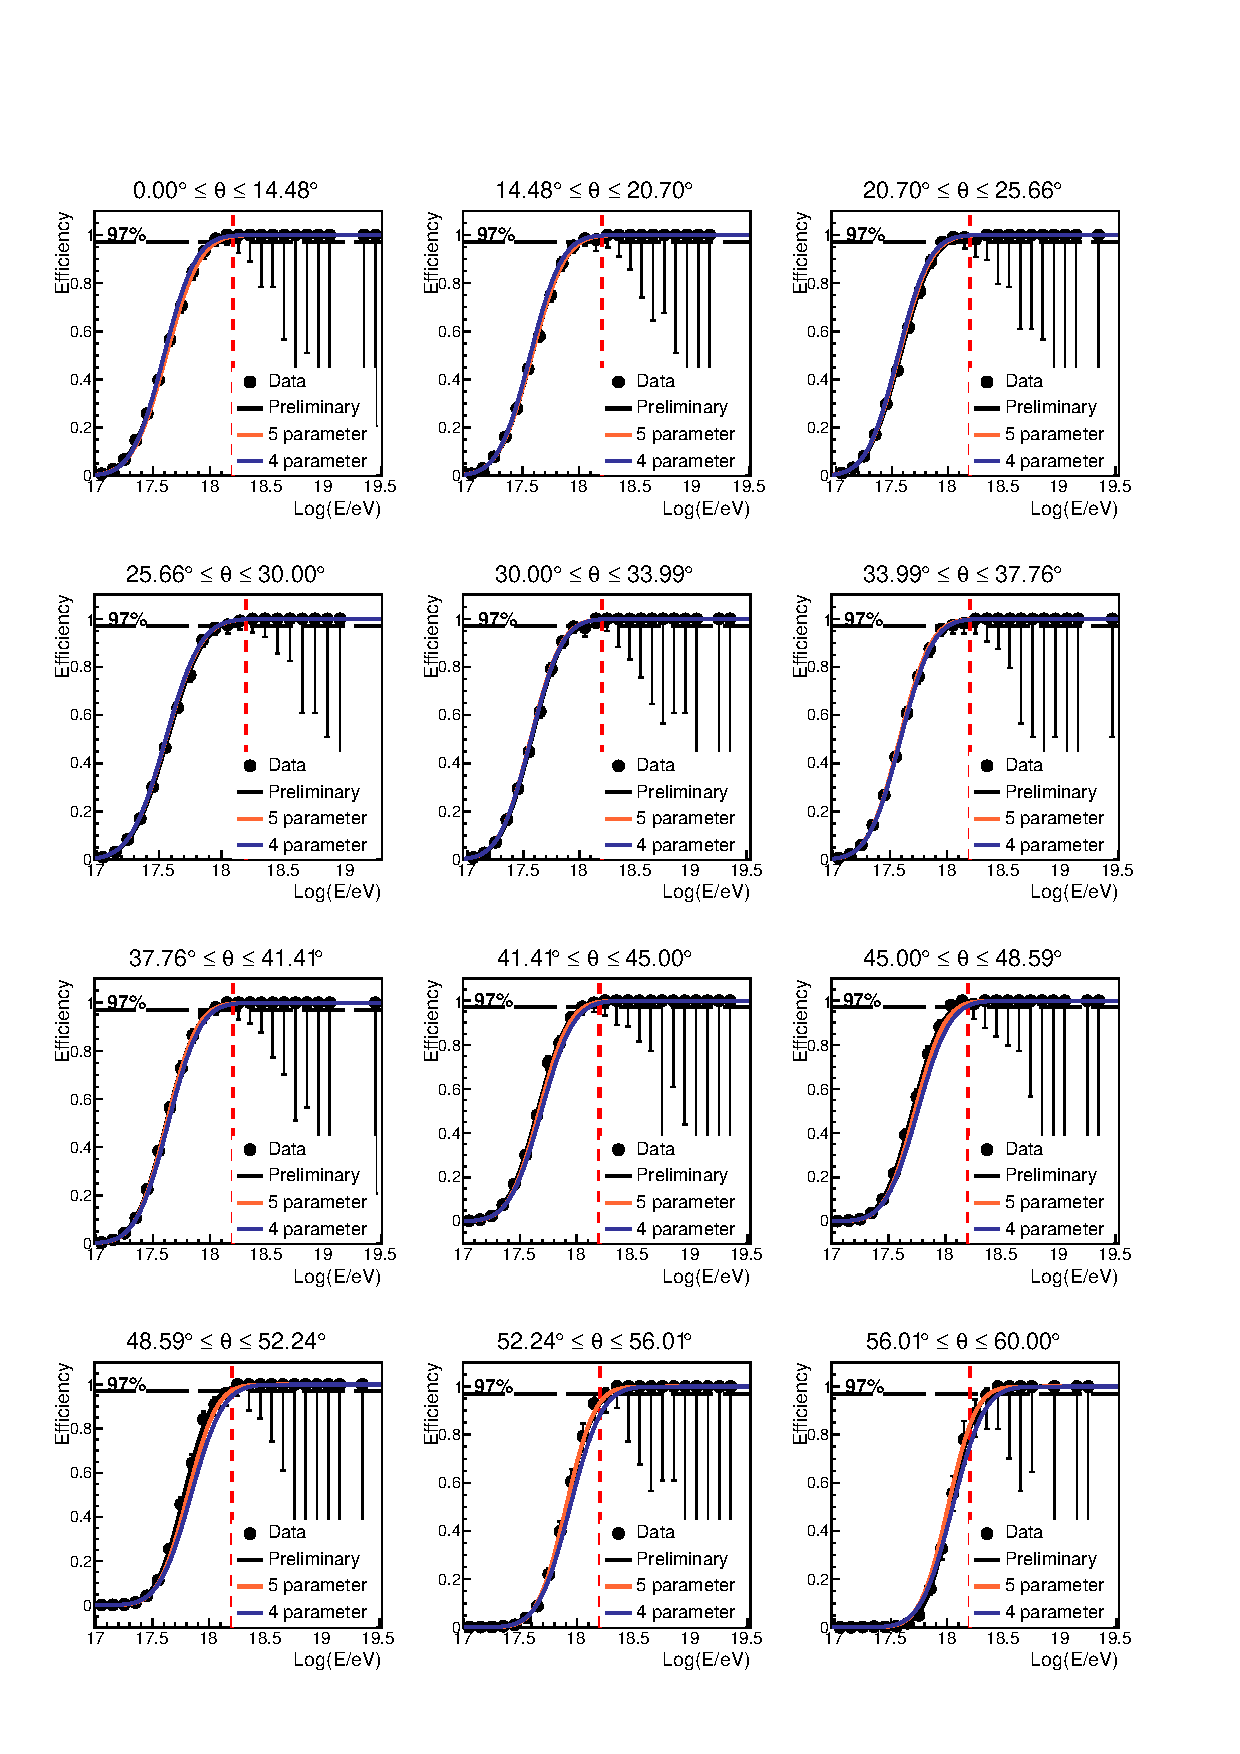
\includegraphics[height=0.9\textheight]{plots/EfficiencyZenithNew.pdf}}
        \caption{Efficiency for the zenith angle bins for events reconstructed including the new triggers and it's parametrizations.
        \label{fig:zenithNew}}
    \end{center}
\end{figure}

\bibliographystyle{plain} % We choose the &quot;plain&quot; reference style
\bibliography{bibliography}

\end{document}
